\chapter{Theoretical Frameworks}

\section{Stratego Game Domain}

Stratego is an imperfect information board game with European roots, popularized in the Netherlands in the 1940s and released in North America in 1961 \cite{perolat2022stratego}. The game is played on a 10x10 board that includes two 2x2 ``lake'' areas in the center, which are impassable. Each player commands an army of 40 pieces of varying ranks, and during the game, the identity and rank of the pieces are kept secret from the opposing player. The objective is to capture the opponent's flag or eliminate all of their movable pieces.

Each army consists of 12 different types of pieces, with ranks ranging from 1 (the Spy) to 10 (the Marshal), alongside Bombs and a Flag. Higher-ranked pieces defeat lower-ranked ones during combat, except in special situations: the Spy can defeat a Marshal if attacking first, the Miner is the only piece that can defuse Bombs, and Scouts can move multiple squares in a straight line. There are 3 ways to win the game capturing the flag, immobilizing all movable enemy pieces, or forcing the opponent to run out of time.


\begin{figure}[ht]
    \centering
    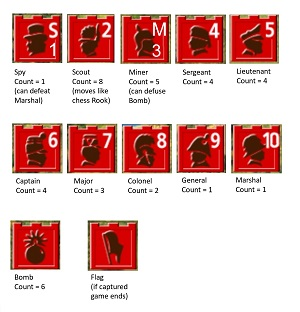
\includegraphics[width=0.5\textwidth]{figures/stratego_piece.png}
    \caption{Stratego pieces.}
\end{figure}

\begin{figure}[ht]
    \centering
    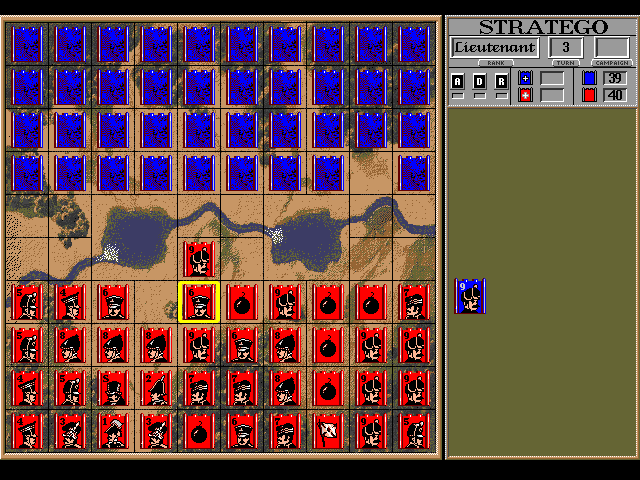
\includegraphics[width=0.7\textwidth]{figures/stratego.png}
    \caption{Stratego Game board.}
    \label{fig:stratego_tech}
\end{figure}

The high theoretical state space of Stratego shows how difficult the game is to solve:

\begin{equation}
|\mathcal{S}| = \binom{40}{1,1,2,3,4,4,4,5,8} \times 10^{10} \times 2^{40} \approx 10^{535}
\end{equation}

Perolat et al. \cite{perolat2022stratego} established the permutation for game state. The agent must use reasoning with limited information rather than trying to look at every possible outcome, making the computation intractable.


\section{MARQ Framework Overview}

The MARQ framework is a Multi-Agent Rainbow Deep Q-Networks system that trains agents through self-play and deep reinforcement learning \cite{AlphaStratego}. Agents learn by competing against many different opponents, including their own previous versions and exploratory variants, within a league-based self-play system.

The central problem is reasoning about hidden information without enumerating every possible state. The number of possible game states exceeds $10^{535}$, and initial setups reach $10^{66}$ per player \cite{perolat2022stratego}. MARQ handles this scale through implicit belief representations, probabilistic reasoning, and pattern recognition. Deep reinforcement learning estimates values. Attention mechanisms process game history. Mixed strategies prevent exploitation. The system keeps all of these computations fast enough to run in real time.

The architecture connects these components in a pipeline. The AAREN module takes raw game positions and move sequences, then produces learned embeddings that encode opponent piece identity inferences. These embeddings form the base for all subsequent reasoning. A league-based training method trains and evaluates MARQ agents simultaneously.



\begin{table}[htbp]
    \centering
    \caption{Key symbols and descriptions.}
    \label{tab:MARQ-symbols}
    \begin{tabular}{|l|p{4cm}|p{6cm}|}
        \hline
        \textbf{Symbol} & \textbf{Description} & \textbf{Example (MARQ Framework)} \\
        \hline
        $\pi_i(a|I_i)$ & Policy for agent i choosing action a given information set $I_i$ & Probability of moving a piece forward given current visible board state and belief about opponent pieces \\
        \hline
        $\mathcal{B}_t$ & Implicit belief representation at time t & Probability distribution over possible identities and positions of hidden opponent pieces inferred by AAREN \\
        \hline
        $v^{\pi}_i(h, \mathcal{B}_t)$ & Value function for agent i following policy $\pi$ given history h and belief $\mathcal{B}_t$ & Expected reward for current board position considering uncertainty about opponent setup \\
        \hline
        $Q_{\text{network}}(s', a)$ & Deep Q-Network approximation of action-value function & Neural network estimate of value for attacking with a suspected Marshal vs opponent piece \\
        \hline
        $R^{\text{capture}}{i,t+1}$ & Immediate reward from piece captures weighted by piece values & +9 points for capturing opponent Marshal, -1 for losing a Scout \\
        \hline
        $O = \{o_1, \dots, o_t\}$ & Observation sequence processed by AAREN attention mechanism & Sequence of board states, moves, and attack outcomes throughout the game \\
        \hline
        $\alpha_i$ & Attention weights for historical observations in AAREN & Higher weight on turn when opponent's Marshal was revealed, lower on routine Scout moves \\
        \hline
        $\pi^*$ & Nash equilibrium policy profile & Optimal mixed strategy that cannot be exploited by opponent strategy changes \\
        \hline
        $Q_{eval}(\mathcal{B})$ & Embedding quality evaluator output & Confidence score for learned representation accuracy \\
        \hline
        $H(\pi)$ & Policy entropy measure & Ensures minimum unpredictability to prevent exploitation \\
        \hline
        $\epsilon$ & Exploration rate for agent behavior & Controls exploration vs exploitation balance in multi-agent learning \\
        \hline
        $\gamma$ & Discount factor for future rewards & Importance of long-term vs immediate rewards in value estimation \\
        \hline
    \end{tabular}
\end{table}


\section{MARQ Policy Definition}

Policy optimization in reinforcement learning improves an agent's strategy to maximize total reward \cite{DRLImperfectInfo2023}. Games with hidden information and multiple players demand policies that perform well against fixed opponents while also handling uncertainty and shifting strategies from other agents. MARQ connects belief state reasoning with value-based decisions to meet these demands.

Policy learning in MARQ serves two goals. The first is winning games through tactical choices. The second is improving the quality of the embeddings that the AAREN module produces. The two objectives reinforce each other: better embeddings sharpen decision-making, and good decisions reveal opponent information that in turn refines the embeddings.

\subsection{Core Policy Framework}

A policy in the MARQ framework, denoted $\pi_i(a|I_i)$, defines a probability distribution over actions for agent $i$ conditioned on its current information set $I_i$. In perfect information games, policies operate on complete game states. MARQ policies do not have that luxury. They reason under uncertainty about the true state of the environment. The information set $I_i$ contains all observations available to the agent: visible board positions, revealed piece identities, and the history of observed movements and combat outcomes.

The core difficulty is that agents must act without knowing the opponent's private information. In Stratego, this means the rank and position of every unrevealed opponent piece remain unknown. The policy must incorporate estimates of the opponent's pieces into its decision process and select actions that perform well across many possible hidden states.

MARQ addresses this by using implicit belief representations $\mathcal{B}_t$ rather than enumerating every possible game state. The AAREN module learns and updates these representations as new information arrives. The policy takes the following form:

\begin{equation}
\pi_i(a|I_i, \mathcal{B}_t) = P(\text{action} = a \mid \text{information set } I_i, \text{implicit belief } \mathcal{B}_t)
\end{equation}

The policy learns to weight actions based on their expected value across the inferred distribution of opponent configurations rather than optimizing for a single specific setup. Playing well requires this kind of reasoning about hidden states.

\subsection{Implicit Representation Optimization}

The quality of the implicit belief representation directly affects decision quality. Inaccurate inferences produce poorly calibrated action values. MARQ therefore treats representation accuracy as an auxiliary training objective and uses revealed piece identities as supervised labels for embedding refinement.

When combat reveals the piece identities, the system calculates the prediction error using Kullback-Leibler (KL) divergence.

\begin{equation}
\mathcal{E}_{\text{pred}}(t) = \sum_{p \in \text{Pieces}_{\text{revealed}}(t)} D_{\text{KL}}\left(\text{Representation}_t(p) \| \delta_{s^*_p}\right)
\end{equation}

Here, $\delta_{s^*_p}$ denotes the Dirac delta distribution concentrated on the true piece type. The error quantifies how far the predicted distribution lies from the actual identity.

This prediction error becomes a representation accuracy reward signal. It encourages the policy to develop embeddings that better predict actual piece configurations:

\begin{equation}
R_{\text{accuracy}}(t) = -\mathcal{E}_{\text{pred}}(t) = -\sum_{p \in \text{Pieces}_{\text{revealed}}(t)} \left[\text{Representation}_t(p=s^*_p) > 0\right] \cdot \log \text{Representation}_t(p=s^*_p)
\end{equation}

The optimal policy maximizes the joint objective of game outcomes and representation accuracy:

\begin{equation}
\pi^*_i = \arg\max_{\pi_i} \mathbb{E}_{\tau \sim \pi_i}\left[\sum_{t=0}^T \gamma^t \left(R_{\text{game}}(t) + \eta \cdot R_{\text{accuracy}}(t)\right)\right]
\end{equation}

The hyperparameter $\eta \in \mathbb{R}^+$ controls the relative importance of representation accuracy versus immediate game rewards.

The value function in MARQ extends the standard Bellman equation to account for belief dynamics. It expresses the expected cumulative reward as a function of the current information set and implicit belief.

\begin{equation}
v^{\pi}_i(I, \mathcal{B}_t) = \mathbb{E}_{\pi}\left[R^{\text{capture}}_{i,t+1} + \lambda_1 R^{\text{info}}_{i,t+1} + \lambda_2 R^{\text{position}}_{i,t+1} + \gamma v^{\pi}_i(I_{t+1}, \mathcal{B}_{t+1}) \mid I_t = I, \mathcal{B}_t\right]
\end{equation}

Three strategic components make up the reward function. The capture reward $R^{\text{capture}}$ reflects material changes. The information reward $R^{\text{info}}$ quantifies the value of information revelation. The position reward $R^{\text{position}}$ measures territorial control.

MARQ training aims to reach a Nash equilibrium. At equilibrium, no player can improve their expected payoff through unilateral deviation. This stability ensures that the policy remains robust against adversarial exploitation.

\begin{equation}
v_i(\pi^*) = \max_{\pi_i} v_i(\pi_i, \pi^*_{-i})
\end{equation}

Finding exact Nash equilibria in large imperfect information games is computationally intractable. MARQ instead seeks approximate equilibria through self-play training with diverse opponent populations.


\section{Deep Q-Network Architecture}

The Deep Q-Networks in MARQ operate on implicit belief representations rather than complete game states \cite{DRLImperfectInfo2023}. The network approximates Q-values over probability distributions of opponent configurations, $\mathcal{B}_t$:
$$Q(s, a) = \mathbb{E}_{s' \sim \mathcal{S}_t \subseteq \mathcal{B}_t}[Q_{network}(s', a)]$$

A standard replay buffer stores experience. Transitions $(\mathcal{B}_t, a_t, r_t, \mathcal{B}_{t+1})$ are sampled uniformly to train the value function.

\subsection{Rainbow DQN Components}
The implementation incorporates several enhancements from the Rainbow DQN architecture \cite{RainbowJMLR2021} to improve stability and sample efficiency.

\paragraph{Distributional RL (Categorical DQN).}
Categorical DQN (C51) models the value distribution directly. It captures the inherent uncertainty of the game by approximating the distribution with 51 atoms spanning the range from $V_{min}$ to $V_{max}$.

\begin{equation}
Z_\theta(s, a) = \sum_{i=1}^{N} p_i(s, a) \delta_{z_i}
\end{equation}
Training minimizes the Kullback-Leibler divergence between the predicted distribution and the projected target distribution:
\begin{equation}
D_{KL}(\Phi \hat{\mathcal{T}} Z_{\theta'} || Z_\theta)
\end{equation}
where $\Phi$ is the projection operator that maps the Bellman update onto the fixed support atoms.

\paragraph{Noisy Networks for Exploration.}
Noisy Linear layers inject learned noise into the network weights. The agent maintains an unpredictable strategy without a separate exploration schedule, and the network itself optimizes the degree of exploration required for each state.

\begin{equation}
y = (\mu_w + \sigma_w \odot \epsilon_w)x + (\mu_b + \sigma_b \odot \epsilon_b)
\end{equation}

\paragraph{Dueling Network Architecture.}
The network separates state value estimation $V(s)$ from advantage estimation $A(s, a)$ using two streams that share a common convolutional feature extractor:
\begin{equation}
Q(s, a; \theta, \alpha, \beta) = V(s; \theta, \beta) + \left( A(s, a; \theta, \alpha) - \frac{1}{|\mathcal{A}|} \sum_{a'} A(s, a'; \theta, \alpha) \right)
\end{equation}
This decomposition improves policy evaluation when many actions carry similar value.

An exploration bonus augments the Q-values. The bonus is based on the uncertainty of the inferred representation, following an optimism-in-the-face-of-uncertainty approach.

\begin{equation}
Q_{augmented}(s, a) = Q_{base}(s, a) + \lambda \cdot U(a)
\end{equation}
Here $U(a)$ represents the entropy of the learned distribution at the target location. This term encourages the agent to investigate unknown opponent pieces.

\subsection{Training Stability via Regularization}

The Ataraxos system reached superhuman performance in no-press Diplomacy, and its designers found that training stability matters as much as the algorithm itself \cite{Ataraxos2025}. Deep reinforcement learning agents face two recurring problems: wasting updates on low-information experiences, and cycling between strategies without settling on a robust one.

\paragraph{Advantage Filtering for Sample Efficiency.}
Advantage filtering concentrates learning on the most informative transitions \cite{RegularizationStrategyExploration}. In reinforcement learning, the temporal-difference (TD) error measures the gap between predicted values and outcomes. A standard replay buffer samples past transitions at random, treating every move equally. Advantage filtering breaks this uniformity. It samples the buffer and retains only the transitions with the largest TD errors:
\begin{equation}
\mathcal{B}_{filtered} = \text{Top}_{n/k}\left(\mathcal{B}_{sampled}, |\delta_i|\right)
\end{equation}
where $\delta_i = r_i + \gamma^n V(s'_i) - V(s_i)$ is the $n$-step TD error for transition $i$.

\paragraph{Dynamic Damping with Power-Law Annealing.}
Strategy cycling is addressed through two regularization terms in the loss function, both based on Kullback-Leibler divergence:
\begin{equation}
\mathcal{L}_{total} = \mathcal{L}_{C51} + \alpha(t) \cdot D_{KL}(\pi \| \pi_{uniform}) + \beta(t) \cdot D_{KL}(\pi_{target} \| \pi)
\end{equation}

The coefficients follow power-law schedules with opposing dynamics:
\begin{align}
\alpha(t) &= \alpha_0 \cdot (1 - t/T)^p \\
\beta(t) &= \beta_0 + (\beta_T - \beta_0) \cdot (t/T)^p
\end{align}
where $t$ is the current episode, $T$ is the total training duration, and $p=2$ produces quadratic curves. Early in training, when uncertainty is highest, the agent explores aggressively. As the policy matures, the schedule shifts weight toward stability.


\section{AAREN and Learned Embedding System}

The AAREN module (Attention as Recurrent Neural Network) \cite{Aaren} serves as the memory and history system within MARQ. It does not maintain simple counts of piece identities. Instead, it produces learned embeddings from opponent moves, and the agent interprets these embeddings through training. AAREN handles long sequences in Stratego. It retains details over hundreds of moves while avoiding the gradient problems that degrade older models such as LSTMs. An attention mechanism lets AAREN look back across the full sequence of moves at once \cite{Aaren}.

\subsection{Recurrent Attention Computation}
AAREN implements an attention-based recurrent computation that maintains a state triplet $(a_t, c_t, m_t)$ across the observation sequence. Traditional recurrent neural networks suffer from vanishing gradients over long sequences. AAREN avoids this entirely. It provides direct access to the full history through attention weights while maintaining $O(1)$ inference complexity per timestep.

Given a sequence of observations $O = \{o_1, \ldots, o_t\}$ where each $o_i$ encapsulates the visible board state and public action outcomes, the AAREN cell first projects each observation into key and value representations:

\begin{equation}
k_t = W_k(o_t), \quad v_t = W_v(o_t)
\end{equation}

The projection matrices $W_k$ and $W_v$ are learned during training. The key $k_t$ determines how relevant the current observation is for belief updates. The value $v_t$ encodes the informational content to be integrated into the belief representation. The attention score $s_t$ measures the relevance of the current observation relative to a learned query vector $q$:

\begin{equation}
s_t = q^T k_t
\end{equation}

The weighted value accumulator $a_t$ aggregates value representations across the sequence:

\begin{equation}
a_t = a_{t-1} \exp(m_{t-1} - m_t) + v_t \exp(s_t - m_t)
\end{equation}

The term $\exp(m_{t-1} - m_t)$ rescales the previous accumulator when a new maximum appears. The term $\exp(s_t - m_t)$ computes the relative attention weight for the current observation. The normalization constant $c_t = c_{t-1} \exp(m_{t-1} - m_t) + \exp(s_t - m_t)$ ensures that the effective attention weights sum to unity. The output $h_t = a_t / c_t$ is an attention-weighted aggregation of all observations up to time $t$.

\subsection{Piece Type Inference}
AAREN infers piece types from action sequences. Each action is encoded as a 24-dimensional feature vector capturing movement patterns, contextual information, and game state features. The network outputs a probability distribution over piece types:

\begin{equation}
P(\text{piece\_type} = t \mid \text{action\_sequence}) = \text{softmax}(W_{out} \cdot h_T + b_{out})_t
\end{equation}

The network combines these embeddings with game rules and the board state to improve decisions under uncertainty.

An evaluation system monitors embedding quality and drives improvement. A neural network evaluator takes embeddings as input and outputs quality scores $Q_{eval}(\mathcal{E}) = \text{MLP}(\mathcal{E}; \theta_{eval})$. Training compares predictions against true piece identities:

\begin{equation}
R_{quality}(\mathcal{B}, g) = \alpha \cdot \mathcal{B}[g] - \beta \cdot |V_{pred} - V_{actual}| - \gamma \cdot \text{distance\_penalty}
\end{equation}

The system decides when additional information gathering is worth the cost through uncertainty assessment:

\begin{equation}
\text{NeedMoreInfo}(\mathcal{B}) = \mathbb{1}\{H(\mathcal{B}) > \theta_H\} \cdot \mathbb{1}\{Q_{eval}(\mathcal{B}) < \theta_Q\}
\end{equation}

\subsection{Embedding Updates on Piece Revelation}

When a battle reveals a piece's true type, the AAREN embeddings synchronize with ground truth. The inferred distribution at the revealed position collapses to certainty:
\begin{equation}
\text{Representation}_{pos}[t] = \begin{cases}
1.0 & \text{if } t = g \\
0.0 & \text{otherwise}
\end{cases}
\end{equation}

The system increments the revealed piece count and adjusts remaining beliefs to respect piece count constraints. For unrevealed positions $p \neq pos$:
\begin{equation}
\mathcal{B}_p[t] \leftarrow \mathcal{B}_p[t] \cdot \frac{\text{max\_count}[t] - \text{revealed\_count}[t]}{\text{remaining\_count}[t]}
\end{equation}

For example, when the single Marshal is revealed, the probability of any other piece being a Marshal drops to zero.

\subsection{Hindsight-Aided Belief Refinement}

The AAREN module provides inference during gameplay. The Hindsight-Aided Belief Refinement (HABR) module adds a second channel: learning from verified information. When combat reveals a piece, HABR applies retrospective learning across the entire history of that piece, using the ground truth as a supervisory signal for past predictions.

\paragraph{Information Gain Reward.}
The Information Gain reward quantifies how much an observation reduces uncertainty about opponent pieces. Let $H(P)$ denote the Shannon entropy of a probability distribution $P$. The KL divergence from a uniform prior $U$ over $N$ piece types is:
\begin{equation}
D_{KL}(P \parallel U) = \log(N) - H(P)
\end{equation}
The Information Gain reward measures the change in this divergence between consecutive representation updates:
\begin{equation}
R_{gain}(t) = D_{KL}(\text{Rep}_{t-1} \parallel U) - D_{KL}(\text{Rep}_t \parallel U)
\end{equation}
Substituting the divergence formula yields:
\begin{equation}
R_{gain}(t) = (\log(N) - H(\text{Rep}_{t-1})) - (\log(N) - H(\text{Rep}_t)) = H(\text{Rep}_{t-1}) - H(\text{Rep}_t)
\end{equation}
$R_{gain}$ equals the reduction in entropy. A positive reward occurs only when the observation at time $t$ increases certainty about piece identity relative to $t-1$. This aligns the agent's incentives with active information gathering.

\paragraph{Sinkhorn Constraint Normalization.}
Independent belief updates for each piece position can produce inconsistent global predictions. Without piece count constraints, the model might assign high probability to multiple pieces being the single Marshal. This phenomenon is called identity inflation. It violates the physical constraints of the game.

Sinkhorn normalization corrects this through iterative proportional fitting. Given a representation matrix $M \in \mathbb{R}^{P \times S}$ where $P$ is the number of tracked pieces and $S$ is the number of piece types, two constraints must hold. The row constraint $\sum_{s} \text{Rep}(p, s) = 1$ ensures each piece has exactly one identity. The column constraint $\sum_{p} \text{Rep}(p, s) = Count(s)$ ensures the total predicted count of each piece type matches the remaining count.

The Sinkhorn algorithm alternates between row and column normalization until convergence. The approach is differentiable, so gradients pass through it. When piece A is confirmed as the Spy, the Sinkhorn layer automatically redistributes probability across all other pieces, creating a shared update across the entire inferred state.


\section{Multi-Agent Learning and Strategy Mixing}

\subsection{League-Based Training Architecture}
The league maintains a changing pool of agents so that the model encounters many different strategies \cite{perolat2022stratego}. The main agent is the best current policy under training. The historical pool stores earlier versions of the main agent, each representing a different stage of development.

Opponents are sampled during training according to a fixed probability distribution.
\begin{equation}
P(\text{opponent}) = 
\begin{cases} 
0.5 & \text{Main Agent (Self-Play)} \\
0.5 & \text{Uniform}(\text{Historical Pool})
\end{cases}
\end{equation}
This prevents the agent from cycling through the same strategies repeatedly. It must defeat all previous versions of itself.

\subsection{Strategy Mixing for Exploitation Resistance}

Deterministic strategies in extensive-form imperfect information games are inherently suboptimal \cite{perolat2022stratego, MARLGametheoretic}. An adversary who knows a deterministic policy reduces the game to a perfect information setting, eliminating the strategic uncertainty that defines games like Stratego. MARQ counters this through two complementary mechanisms.

At the action selection level, Noisy Linear layers inject learned, state-dependent noise into the policy. The network learns the appropriate degree of randomization for each game state rather than relying on fixed exploration schedules such as $\epsilon$-greedy.

At the strategy level, diverse opponent exposure during training achieves mixing. The league system maintains a population of historical agent checkpoints, each representing a different strategic approach discovered during training. Action randomness combined with strategy variety produces policies that are unpredictable and resistant to exploitation.

\subsection{Multi-Dimensional Reward Structure}

The reward function $R(s, a, s')$ guides learning in Stratego's sparse-reward environment \cite{PBRSModern2022}:

\begin{equation}
R_{total} = R_{move} + R_{capture} + R_{tactical} + R_{info}
\end{equation}

The move reward $R_{move}$ gives small bonuses for advancing pieces (approximately $+0.05$) to encourage active play. The capture reward $R_{capture}$ scales by the rank of the captured piece according to $0.15 \times \frac{\text{Rank}}{11.0}$. The tactical reward $R_{tactical}$ assigns specific bonuses for key strategic captures: $+0.5$ for Miner vs Bomb defusals and $+1.0$ for Spy vs Marshal assassinations. The information reward $R_{info}$ provides $+0.3$ for revealing high-value opponent pieces.

The framework uses \textit{Reward Annealing} to transition from tactical learning to strategic gameplay. Dense shaping rewards are scaled down as the training curriculum advances. In later training phases, these auxiliary signals are completely removed, and the agent relies exclusively on sparse, terminal win/loss rewards. This progression prevents the agent from developing sub-optimal behaviors driven by short-term shaping incentives.


\section{Specialized Agent Architectures}

\subsection{Setup Agent via Distributional RL}

A specialized SetupAgent handles the game's initial setup. It learns optimal piece configurations by treating the placement phase as a sequential decision process. The state representation is a 3-channel input tensor: one channel encodes the current board state with already-placed pieces, a second provides a valid positions mask indicating legal placement locations, and a third identifies which piece type is currently being placed.

The agent outputs a distributional Q-value for each of the 100 board positions, mapping $Q(s, pos)$ to a distribution over $[V_{min}, V_{max}]$. This distributional approach captures the inherent uncertainty in setup quality, since the true value of a placement depends on the unknown opponent configuration.

An exploitability critic network penalizes predictable placements to prevent static, easily countered setups:

\begin{equation}
\mathcal{L}_{total} = \mathcal{L}_{C51} + \lambda \cdot \mathcal{L}_{predictability}
\end{equation}


\subsection{Information Set Monte Carlo Tree Search (IS-MCTS)}

For high-stakes decisions, especially in the endgame, MARQ uses an Information Set MCTS agent \cite{UpdatedISMCTS} that combines search with learned value functions. The search operates in three phases.

In the determinization phase, the agent samples a consistent concrete world state $s_{det}$ from the history-based beliefs according to $s_{det} \sim P(S | \mathcal{B}_t)$. This converts the imperfect information game into a perfect information instance for the duration of the simulation.

In the tree traversal phase, a UCB1 variant navigates the search tree to balance exploration and exploitation of move sequences. Nodes represent information sets rather than individual states, so the tree can be shared across multiple determinizations.

In the leaf evaluation phase, terminal or unexpanded nodes are evaluated using the Rainbow DQN value function instead of random rollouts:

\begin{equation}
V(s_{leaf}) \approx Q_{DRQN}(s_{leaf}, a_{best})
\end{equation}


\section{Game Environment and State Management}

The Stratego environment provides the foundation for agent training and evaluation. It manages the complex dynamics of imperfect information.

\subsection{Information Set Management}
The environment maintains distinct representations for each information context:

\begin{equation}
\mathcal{I}_{player} = \{s : s \text{ is consistent with player observations}\}
\end{equation}

Each player receives only the subset of game state information available through its observation function.

\subsection{Temporal State Evolution}
Game states evolve according to an update function.

\begin{equation}
s_{t+1} = \text{EnvStep}(s_t, a_t^1, a_t^2, \theta_t)
\end{equation}

Here $\theta_t$ represents stochastic elements such as hidden information revelation and time limits.

\subsection{Valid Action Filtering}
The environment enforces game rules through valid action constraints:

\begin{equation}
\mathcal{A}_{valid}(s, player) = \{a : \text{IsLegalMove}(a, s, player) \land \text{RespectsGameRules}(a, s)\}
\end{equation}

Only legal moves consistent with Stratego's rules and piece capabilities are available to the agent.

\subsection{Piece Setup and Initialization}
Setup policies govern strategic piece placement.

\begin{equation}
\pi_{setup}(\text{placement}|player) = \text{NeuralNetworkSetup}(\text{strategic\_features}, \theta_{setup})
\end{equation}

Strategic features include positional value maps, piece interaction potentials, and defensive vulnerabilities. The initial placement of pieces is a high-impact decision that shapes the remainder of the game \cite{PlacementSetup}.

\section{MARQ Move Selection and Decision-Making}

The MARQ framework's architectural components converge in the real-time move selection process. Algorithm \ref{alg:marq_decision} details this procedure, which integrates learned positional priors with tactical search to optimize behavior in adversarial environments.

\begin{algorithm}
\caption{MARQ: Decision-making and Move Selection}
\begin{algorithmic}[1]
\REQUIRE Public Observations $O$, Board State $S$, DQN weights $\theta$, AAREN weights $\phi$, Temperature $T$
\ENSURE Optimal Action $a^*$
\STATE $\mathcal{H}_t \gets \text{UpdateAggregation}(O, \phi)$ 
\STATE $\mathcal{B}_t \gets \text{GetSoftmaxBeliefs}(\mathcal{H}_t)$ 
\STATE $X_t \gets \text{Concatenate}(S, \mathcal{H}_t)$ 
\STATE $Q(s, \cdot) \gets \text{RainbowInference}(X_t, \theta)$ 
\STATE $\mathcal{A} \gets \text{LegalMoves}(S)$
\FORALL{$a_i \in \mathcal{A}$}
    \IF{$\text{IsAttack}(a_i, S)$}
        \STATE $target\_pos \gets \text{TargetSquare}(a_i)$
        \STATE $P \gets \mathcal{B}_t(target\_pos)$ 
        \STATE $V_{exp} \gets \sum_{r \in \mathcal{R}} P(r) \cdot \mathbb{U}(\text{Attacker}, r)$ 
        \STATE $V_{final}(a_i) \gets \lambda Q(s, a_i) + (1-\lambda) V_{exp}$
    \ELSE
        \STATE $V_{final}(a_i) \gets Q(s, a_i)$
    \ENDIF
\ENDFOR
\IF{Training/Self-Play and $T > 0$}
    \STATE $\pi(a_i) \gets \frac{\exp(V_{final}(a_i) / T)}{\sum_{a \in \mathcal{A}} \exp(V_{final}(a) / T)}$
    \STATE \textbf{return} $a^* \sim \pi(\cdot)$
\ELSE
    \STATE \textbf{return} $a^* \gets \arg\max_{a_i \in \mathcal{A}} V_{final}(a_i)$
\ENDIF
\end{algorithmic}
\label{alg:marq_decision}
\end{algorithm}

\subsection{Historical Context Update}
The decision process begins with the AAREN module's recurrent attention system. As game observations arrive, the history aggregator updates its internal state. The agent's current embedding thus reflects the opponent's cumulative behavioral patterns, not just the immediate board state.

\subsection{Probabilistic Belief Extraction}
After updating the history, the system extracts softmax probability distributions for hidden pieces. These piece-identity predictions are generated for every square on the board. They represent the agent's current belief about the hidden ranks of unrevealed opponent pieces.

\subsection{Information Set Tensorization}
The visible board state and the learned AAREN embeddings are concatenated to form a high-dimensional information set representation. In the current implementation, this produces a 79-channel input tensor (15 physical board features + 64 history embedding channels), which encapsulates both the physical layout and the inferred hidden context.

\subsection{Value Distribution Estimation}
The Rainbow DQN's convolutional backbone and C51 distributional head process the 79-channel tensor. This step estimates the $Q$-value distribution over 51 atoms for all possible actions. The distribution captures the multi-modal uncertainty inherent in the state.

\subsection{Action-Space Filtering}
Legal move masking ensures rule compliance and efficiency. The Q-network's output is filtered against the set of valid moves $\mathcal{A}$ defined by Stratego's rules. Illegal actions cannot be selected.

\subsection{Expectamax Search and Tactical Summation}
Standard adversarial search algorithms like Minimax assume an opponent who plays optimally to minimize the agent's utility. Many environments involve stochastic elements or hidden information that are better modeled as probabilistic transitions \cite{DRLImperfectInfo2023, SubgameSolving2021}. Algorithms addressing this class of problems introduce ``Chance Nodes'' into the game tree.

In Stratego, the identity of an opponent piece encountered during an attack is a stochastic variable. The Expectamax value is an exact summation over the rank probabilities provided by the belief extractor: 
\begin{equation}
\mathbb{E}[V] = \sum_{r \in \mathcal{R}} P(\text{target is rank } r) \cdot \mathbb{U}(\text{outcome vs } r)
\end{equation}
The agent can pursue tactical aggression when the probability of a successful capture outweighs the risk of piece loss. The decision is grounded in the AAREN's inference history.

\subsection{Stochastic Action Selection (Temperature Scaling)}
Rigid, exploitable behavior loops must be avoided during self-play and evaluation. The final action selection step uses Temperature Scaling (Boltzmann Options). Instead of choosing the action with the highest expected value via a hard \textit{argmax}, the agent samples from a stochastic softmax distribution parameterized by a temperature variable $T$. The probability of selecting action $a_i$ follows the Boltzmann distribution over the action values $V_{final}$:
\begin{equation}
\pi(a_i) = \frac{\exp\left(V_{final}(a_i) / T\right)}{\sum_{a \in \mathcal{A}} \exp\left(V_{final}(a) / T\right)}
\end{equation}
As $T$ approaches zero, the selection becomes deterministically greedy. When $T$ increases, near-optimal actions receive proportionally higher selection probabilities, injecting controlled variance. This stochasticity serves two purposes: it generates a diverse and unpredictable curriculum roster during league training, and it prevents tactical stagnation within recurring positional maneuvers.

\section{Generalizability}

The MARQ framework provides mathematical stability in adversarial settings and applicability to real-world domains beyond gaming. This section presents the convergence guarantees of the training methodology and the potential for transferring learned representations to non-gaming environments.

\subsection{Mathematical Convergence Properties}
MARQ provides theoretical guarantees for convergence and performance under specific conditions.

\subsubsection{Incremental Learning Bounds}
The algorithm bounds value function estimation error as follows:
\begin{equation}
\|V_t - V^*\|_\infty \leq \frac{C}{\sqrt{t}} + \epsilon_{approx}
\end{equation}
where $C$ depends on reward bounds and the discount factor, and $\epsilon_{approx}$ represents function approximation error.

\subsubsection{Implicit Representation Accuracy Bounds}
Representation accuracy improves with additional observations:
\begin{equation}
\mathbb{E}[\text{Accuracy}(\mathcal{B}_t)] \geq 1 - \exp(-\alpha \cdot N_{obs}(t))
\end{equation}
where $N_{obs}(t)$ is the cumulative number of informative observations and $\alpha$ is a positive constant.

\subsubsection{Strategy Convergence in Self-Play}
The league training methodology converges to $\epsilon$-Nash equilibria under standard monotonic improvement assumptions:
\begin{equation}
\lim_{T \to \infty} \| \pi_T - \pi^* \| \leq \epsilon
\end{equation}
for some $\epsilon > 0$ depending on the exploration parameters and opponent diversity. Hierarchical best-response maintenance, main-pool promotion thresholds, and diversity-driven exploration drive this convergence.

\subsection{Applied Generalizability}
The MARQ framework was developed for Stratego, but its architecture applies to broader problems involving partial observability and adversarial decision-making.

\subsubsection{Inference in Degraded Environments}
The occlusion-based curriculum combined with AAREN history aggregation provides a method for training agents to operate in degraded environments. In autonomous drone applications, sensors may fail or be obstructed by smoke or weather. MARQ's ability to maintain an implicit belief state allows continued navigation and objective completion despite sensor loss.

\subsubsection{Signal Intelligence and Pattern Discovery}
In adversarial signal environments such as electronic warfare, implicit representation learning can discover latent identities in high-dimensional signal data. The network treats signal history as an action sequence and learns to categorize threats without explicit labeling of every transmission.

\subsubsection{Industrial Automation and Predictive Maintenance}
MARQ's architecture can integrate sparse sensor readings over time to predict hidden anomalies or maintenance needs in complex manufacturing pipelines. This enables proactive adjustments before system failure occurs.

These convergence properties and the transferability of the learned embeddings support confidence in the framework's ability to handle high-stakes gameplay and transition to practical applications.

%\section{AI Transparency, Inclusion, and Originality of Intent}

%The development of the MARQ framework for Stratego was governed by intentionality and human-led architectural design. While large language models and generative AI have become ubiquitous in modern software development, their role in this research was strictly limited to tasks such as grammatical refinement, high-level brainstorming, and code debugging for modules and networking. Every core component of the MARQ system, including the AAREN history aggregator and the ResNet-based policy heads, was researched, evaluated, and implemented with the intent of mastering imperfect information games in the Stratego domain.

\section{Algorithmic Evolution and Architecture Ablations}

The final MARQ architecture emerged from systematic experimentation and the refinement of several reinforcement learning components. Multiple established algorithms were evaluated and replaced because of performance bottlenecks or insufficient strategic depth in the Stratego domain.

\paragraph{Value Optimization and Exploration.} 
Early iterations used a normal DQN with $\epsilon$-greedy exploration. This approach proved inadequate for Stratego's sparse rewards and led to early stagnation. The implementation was upgraded to a Rainbow DQN architecture incorporating Noisy Networks for state-dependent exploration. The standard double-DQN configuration was then replaced with a Dueling Head architecture, which improved value estimation accuracy in states where multiple actions carry similar utility. To mitigate overfitting to deterministic opponent policies during self-play, the system also employs \textit{Boltzmann Exploration} (Temperature Scaling). The opponent's action selection uses a temperature-scaled softmax over Q-values, injecting controlled stochasticity to produce a more robust training curriculum.

\paragraph{History and Memory Representation.} 
Initial attempts to manage hidden information relied on explicit Probabilistic Belief States. These states introduced prohibitive computational complexity and memory overhead. They required $O(N^2)$ updates that throttled training throughput. The framework moved to an implicit belief system powered by the AAREN architecture. Long Short-Term Memory cells for trajectory embeddings were also replaced by AAREN's attention-based recurrence, which provided more stable gradient flow over long sequences and better handled the non-Markovian nature of piece identity inference.

\paragraph{Architectural Refinements.} 
The convolutional backbone underwent several iterations, moving from standard deep convolutional stacks to a dedicated ResNet architecture. Testing identified 6 Residual Blocks as the optimal depth. This configuration provides full receptive field coverage of the 10x10 board while maintaining low inference latency. The optimizer was transitioned from standard ADAM to ADAMW to improve weight decay and policy loss stability.

\paragraph{Strategic Initialization and Efficiency.} 
The piece placement phase was initially modeled using an agentic SetupAgent trained through distributional reinforcement learning. This approach introduced exploitability risks and operational overhead. The project transitioned to a non-agentic, fixed Heuristic Setup Agent with randomized flag positioning. The change resolved the exploitability concern and provided substantial computational savings. The agentic setup required approximately 2 seconds per episode; the heuristic method completes in under 100 milliseconds. This optimization effectively halved the total training compute requirement.
